% -*- coding: utf-8 -*-
% !TeX encoding = UTF-8
% !TeX root = ../report.tex


%% kunne være en ide at inkludere den sort-hvide udgave af det endelige moneca kort, bare så de kan se hvad pokker det egentligt handler om. Sætte det ind i starten som en lille figur.


%%%%%%%%%%%%%%%%%%%%%%%%%%%%%%%%%%%%%%%%%%%%%%%%%%%%%%%%%%%
\chapter{Moneca: Jobmobilitet og klyngedannelse \label{kap metode_sna}}
%%%%%%%%%%%%%%%%%%%%%%%%%%%%%%%%%%%%%%%%%%%%%%%%%%%%%%%%%%%

Den primære metode i dette speciale er en social netværkanalytisk tilgang til jobmobilitet på arbejdsmarkedet. Ud fra en beslutningsprocedure - algoritme, om man vil - baseret på centrale mål indenfor netværksteori, skabes der klynger af jobs, hvori mobiliteten mellem dem er særlig hyppig. Dette kapitel vil gennemgå denne metode. Målet er at give læseren en forståelse af, hvordan klyngedannelsen i Moneca finder sted. Da der er tale om en ny måde at bruge social netværksanalyse på, bygget på netværksanalytiske mål, er der ikke andet litteratur på metoden end de to artikler fra skaberne af metoden, Toubøl og Grau Larsen. Samt et speciale af Nielsen-Gravholt, som jeg samarbejdede med i dataindsamlingen og brugen af metoden. 


Gravholt-Nielsen og jeg er dermed de første, der benytter sig af metoden, og udover de to der udviklede den. Denne afhandling er dermed også et eksplorativt metodeforsøg, der må holde sig metodens tidlige udviklingsstadie for øje. Det betyder, at jeg i mit arbejde har brugt meget tid på at sikre mig dens resultater, og forstå dens logik. Dette fremgår ikke nødvendigvis af teksten i afhandlingen, hvilket det heller ikke bør gøre. Det er dog centralt at forstå, at netop på grund af metodens uprøvede karakter, blev det, og bliver det, vigtigt at fastslå, hvad den “kan bruges” til, for nu at tale i fra-forskning-til-faktura sprog, hvilket er ganske fornuftigt i nogle sammenhænge.

Et delmål for dette speciale er derfor at undersøge, hvad Moneca-algoritmen er i stand til, samt være opmærksom på dens eventuelle begrænsinger og mulige fejlbehæftninger. Dette vil løbende blive diskuteret i specialet.

først vil jeg... Lorem ipsum dolor sit amet, consectetur adipisicing elit, sed do eiusmod
tempor incididunt ut labore et dolore magna aliqua. Ut enim ad minim veniam,
quis nostrud exercitation ullamco laboris nisi ut aliquip ex ea commodo
consequat. Duis aute irure dolor in reprehenderit in voluptate velit esse
cillum dolore eu fugiat nulla pariatur. Excepteur sint occaecat cupidatat non
proident, sunt in culpa qui officia deserunt mollit anim id est laborum.

 % Det er derfor et delmål for dette speciale at evaluere hvorledes Moneca fungerer i relation til videnskabelige mål for reliabilitet og validitet. 



%%%%%%%%%%%%%%%%%%%%%%%%%%%%%%%%%%%%%%%%%%%%%%
\section{et pragmatisk, videnskabsteoretisk udgangspunkt: relationel sociologi som værktøj \label{videnskabsteori} }
%%%%%%%%%%%%%%%%%%%%%%%%%%%%%%%%%%%%%%%%%%%%%%

Den centrale forskel, som eksempelvis Mustafa Emirbayer fremhæver i sit manifest for en relationel sociologi \citeyear{Emirbayer1997}, er at det, der skaber enshed i en social gruppe, er hvorvidt der eksisterer en forbindelse mellem aktører, altså relationelle størrelser. Fremfor at de grupperes efter givne attributter,
Det princip, klyngedannelsen er baseret på, er dermed hvorvidt der eksisterer en forbindelse mellem klyngens medlemmer, altså en relationel størrelse. Hvorimod en substantialistisk metode ville benytte sig af givne attributter, til at gruppere en række aktører, uden at dette nødvendigvis indebar nogen enshed. 

Emirbayer mener, at det primære valg enhver sociolog må træffe ”\emph{(…) is the choice between substantialism and relationalism}” \parencite[282]{Emirbayer1997}. Den substantiele sociologi bygger på en opfattelse af, at sociale enheder bredt forstået har en egenværdi i form af nogle indre kvaliteter, der er udgangspunkt for deres påvirkning af verden omkring dem \parencite[282f]{Emirbayer1997}. 

Dette er måske noget skarpere skårent, end jeg 

Vi vil i dette projekt ikke tage stilling for eller imod den relationelle og den substantiele tilgang så emfatisk, som Emirbayer kræver det i sit manifest. Vi argumenterer i stedet for at disse to tilgange i højere grad repræsenterer poler i et kontinuum. Dette kontinuum går fra en ren relationel tilgang, hvor alle kvaliteter opstår i relationer til en ren substantiel tilgang, hvor alle egenskaber måles som indre og fikserede, og den rene version af den ene pol kan være lige uhensigtsmæssig at arbejde med som den anden. 
Scott gør det muligt at arbejde med et sådant kontinuum ved at forstå variabelbaseret analyse og netværksanalyse som to metodiske greb, der kan bruges komplementært \parencite[3ff]{Scott2000}. I stedet for at anse disse to metodologiske tilgange som to adskilte ontologier, ser Scott dem som forskellige slags analyser, der afhænger af datamaterialet. Netværksanalyse kræver relationel data, mens variabelanalyse kræver attributbaseret data. Dermed er der ikke tale om et valg om, hvordan den sociale virkelighed ser ud, men et spørgsmål om, hvilken type undersøgelse man ønsker at foretage. Måden, man forholder sig til et givent socialt fænomen, bør som følge heraf basere sig på en bevidst vurdering af, hvad der er mest hensigtsmæssigt for den konkrete undersøgelse.






%%%%%%%%%%%%%%%%%%%%%%%%%%%%%%%%%%%%%%%%%%%%%%
\section{Arbejdsmarkedet som et netværk \label{sec_}}
%%%%%%%%%%%%%%%%%%%%%%%%%%%%%%%%%%%%%%%%%%%%%%

Arbejdsmarkedet bliver her forstået som et netværk af forskellige arbejdsstillinger. Hvad der skaber forbindelser mellem arbejdstilingerne, er jobskifte.  Det sker når en person går fra at være beskæftiget i en arbejdsstilling til at være beskæftiget i en anden arbejdsstilling. Arbejdsstillingerne altså betragtes som \emph{noder} i et netværk, og personernes bevægelser mellem forskellige arbejdsstillinger bestemmes som \emph{forbindelserne mellem} noderne . Netværket er \emph{vægtet}, det vil sige en forbindelse mellem to noder/arbejdstillinger ikke bare en forbindelse: Den har en bestemt værdi, der beskriver hypigheden af skift mellem de pågældende noder.

Moneca er kort sagt en beslutningsprocedure, der bestemmer, hvordan noderne skal grupperes, baseret på styrken af forbindelserne. Deraf navnet: \emph{Mobility Network Clustering Algorithm}, Moneca.

Det er en kvantitativ, \emph{deskriptiv} metode, hvis formål kan opsummeres til: 
%
\begin{enumerate} \label{monecaformaal}
  \item at vise tilstedeværelsen, fraværet og styrken af forbindelser mellem noder.
  \item Benytte et sæt kriterier/beslutningsregler til at bestemme en klyngedannelse af noder, baseret på centrale mål indenfor graf-teori%
  %
  		\footnote{ \emph{Graf-teori} er et andet term for netværksanalyse, hvis semantik mere betoner det matematiske fundament, der bruges til at analysere netværket.}%
  %
\end{enumerate}
%

Hvad noderne er bestemmes ud fra det empiriske formål. Toubøl og Larsen har benyttet Moneca til at se på den sociale mobilitet mellem forskellige beskæftigelseskategorier indenfor hele det danske arbejdsmarked. Jeg har benytter således Moneca til det samme formål som dem, omend på en noget anden måde, og med et speciale til rådighed, noget mere plads til at udfolde analysen, end to artikler i tidskrifter muliggør. 

%
\subsection{ Mobilitetstabel \label{subsec_}}
%

Mit udgangspunkt for dannelsen af netværket er en såkaldt mobilitetstabel. Denne viser skift fra beskæftigelseskategorierne i rækkerne til beskæftigelseskategorierne i kolonnerne. Det er illustreret i tabel \ref{tab_adjacencyeks}%
%
		\footnote{ Tallene er fiktive.}%
%


%
\begin{table}[H] \centering
\caption{Eksempel på en adjacency matrice}
\label{tab_adjacencyeks}
\resizebox{0.8\textwidth}{!}{%
\begin{tabular}{@{}l|cccc@{}} \toprule
	                & Til: Tandlæge & Til: Folkeskolelærer & Til: Pædagog & Til: Automekaniker \\ \midrule
	Fra: Tandlæge        & 264      & 0               & 0       & 0             \\ 
	Fra: Folkeskolelærer & 0        & 6148            & 288     & 6             \\ 
	Fra: Pædagog         & 0        & 454             & 9308    & 0             \\ 
	Fra: Automekaniker   & 0        & 13              & 13      & 1861          \\ \bottomrule
\end{tabular} }
\end{table}
% 

I netværkstermer kaldes sådan en tabel for en \emph{adjacency matrice}, da den har samme udfald i både rækker og kolonner. Således er datamatricen kvadratisk \parencite[55]{Scott2000}. At der er tale om en mobilitetstabel betyder, at rækkeudfaldene er de beskæftigelseskategorier, personer på arbejdsmarkedet kommer \emph{fra}, og kolonneudfaldene er de beskæftigelseskategorier, disse personer er gået \emph{til}. 

Det ses at 264 personer på et tidspunkt har skiftet fra tandlæge til tandlæge i løbet af de 14 år, og ikke har skiftet til nogle af de andre tre erhverv. Skift fra samme beskæftigelse til samme beskæftigelse forekommer langs diagonalen, og har derfor en anden betydning end de andre skift: Her er der tale om den \emph{interne jobmobilitet}. 

En mobilitetstabel som denne er en \emph{retningsbestemt}, \emph{vægtet} adjacency matrice, hvilket er den mest komplicerede form for  data i social netværksanalyse \parencite[61]{Scott2000}. 


\underline{vægtet} betyder at de enkelte celler ikke tilkendegiver en binær opdeling i tilstedeværelse eller fravær af en forbindelse, eksempelvis mellem folkeskolelærer og automekaniker, men at den også angiver en værdi for styrken, eller hyppigheden, af denne forbindelse. 

\underline{Retningsbestemt} betyder at matricen ikke er symmetrisk på diagonalen: Der er forskel på at gå fra tandlæge til folkeskolelærer, og gå fra folkeskolelærer til tandlæge. Derfor er matricen ikke symmetrisk på diagonalen. I en \emph{vægtet} retningsbestemt matrice kan der være forskel i hyppigheden mellem at gå fra tandlæge til folkeskolelærer og folkeskolelærer til tandlæge. 


I tilfældet automekaniker ses det, at hvis man i matricens nederste del kigger på automekaniker, er relationen til tandlæge 0, det vil sige fraværende, mens den til folkeskolelærer og pædagog har en styrke på 13 i begge tilfælde. I selve diagonalen, det  vil sige \emph{den interne mobilitet} for automekanikere, er styrken langt højere. Hvis man ser på hvor automekanikere skifter job til, i matricens nederste del, skal matricen aflæses kolonnevis: det vil sige der er ingen forbindelse til tandlæge, en styrke på 13 til folkeskolelærerer, det samme til pædagoger, og en intern mobilitet på 1861. Det viser, hvad der menes med en retningsbestemt, vægtet adjacency matrice: Styrken i mobiliteten fra automekaniker til folkeskolelærer er på 13, mens den fra pædagog til automekaniker er på 6, altså halvt så kraftig.



%%%%%%%%%%%%%%%%%%%%%%%%%%%%%%%%%%%%%%%%%%%%%%%%%%%%%%%%%%%
\subsection{Relativ risiko og styrken af forbindelser \label{metode_relativrisiko}}
%%%%%%%%%%%%%%%%%%%%%%%%%%%%%%%%%%%%%%%%%%%%%%%%%%%%%%%%%%%

Indtil videre har jeg kun talt om styrken af forbindelser som antallet af skift mellem job. Det er en måleenhed, der repræsenter ét menneskes skift én gang mellem to job.. Det er imidlertidig ikke altid retvisende, da styrken af forbindelsen dermed ikke er relativ til antallet af personer beskæftiget i erhvervet. I 1996 var der eksempelvis 5.207 tandlæger, mens der var 53.676 beskæftigede pædagoger, altså omtrent ti gange så mange. Et skift fra tandlæge til en anden profession bør derfor vægtes højere end et skift fra pædagog til en anden profession.  Her kommer konceptet relativ risiko ind i billedet, som en ratio mellem to proportioner \parencite[244, 271]{Agresti1997}: 
%
\begin{align} 
\frac{\pi_{A}}{\pi_{B}}
\end{align} 
%
Den relative risiko (RR) fortæller os hvad chancen er for at begivenhed B sker, relativt til begivenhed A. Begivenhed A kender vi. Det er den simultane sandsynlighed for udfald \emph{x} og udfald \emph{y} i de to stokastiske variable \emph{I} og \emph{J} () \parencite[41]{Malchow-MoellerWuertz2010}, givet ved sandsynlighedsfunktionen:
%
\begin{align} 
f(i,j) = P(I=i, J=j)
\end{align} 
%
I eksemplet fra tabel \ref{tab_adjacencyeks} er den simultane sandsynlighed for at have skiftet fra folkeskolelærer til pædagog: $\frac{45}{45} = 0,45 = \pi_{A}$. Begivenhed B er til vores formål%
%
\footnote{Indenfor medicinsk forskning vil relativ risiko typisk blive brugt sammen med oddsratio-værdier til at bestemme risici mellem en gruppe patienter tildelt en ny medicin samt en kontrolgruppe. Relativ risiko bruges typisk til at vurdere forskelle mellem to reelt eksisterende grupper. Toubøl og Larsen benytter det i stedet som det bruges indenfor hypotesetest som det kommer til udtryk i eksempelvis $\chi^{2}$-testen \parencite[205]{Malchow-MoellerWuertz2010}, det vil sige, hvor vi har en teoretisk forventet værdi for en bestemt gruppe.}% 
%
karakteriseret som \emph{den forventede værdi}. Det er en teoretis værdi, der er bestemt ud fra en forventning om hvad chancen \emph{bør være} for at begivenheden indtræffer, ud fra bestemte forudsætninger. Hvad er så disse forudsætninger?

Toubøl \& Larsen foreslår at det forventede udfald $\pi_{B}$ bør være uafhængighed mellem f(I) og f(J).

Hvis vi antager at arbejdsmarkedet er et frit marked, er der således tale om den perfekte markedstilstand, uden nogen barrierer eller flaskehalse; alle søger til og fra jobs som man bør forvente ud fra fordelingen af de givne jobs, og det uden at være betinget af hvilke jobs man kommer fra.

Eller i matematiske termer: uafhængighed mellem to variable indebærer at de marginale sandsynligheder for \emph{I} og \emph{J} giver den simultane sandsynlighed \parencite[43f]{Malchow-MoellerWuertz2010}:
%
\begin{align} \label{eq_ss_under_uafh} 
f(i,j) = f_{J}(i)*f_{J}(j)
\end{align} 
%

Den eneste betingelse er, som nævnt før, den, at den relative frekvens for begge variable har betydning for fordelingen: Der tages højde for, om der kun findes 5 slagtere i Danmark, og 10.000 urmagere.

Lad $\pi_{ij_{B}}$ være udtrykket for den simultane sandsynlighed under uafhængighed for den \emph{i}de række og den \emph{j}de kolonne, det jeg i starten benævnte som begivenhed B. $\pi_{ij_{A}}$ er den observerede simultane sandsynlighed der observeres: f(\emph{i},\emph{j}). Den relative risiko, beregnet ud fra de observerede marginale sandsynligheder, er derved givet ved udtrykket   
%
\begin{align} \label{eq_RR_observeret1}
% f(i,j) = f_{J}(i)*f_{J}(j)
\frac{\pi_{ij_{A}}}{\pi_{ij_{B}}} = \frac{f(i,j)}{f_{I}(i)*f_{J}(j)} = RR_{(i,j)_{observeret}}
\end{align} 
%
Det betyder, at hvis den relative risiko for celle(\emph{i,j}) er lig 1, er formel \ref{eq_ss_under_uafh} sand, og dermed eksisterer der uafhængighed mellem job \emph{i} og job \emph{j}. Hvis RR er under 1, er sandsynligheden for jobskifte mellem de to jobtyper mindre end forventet givet uafhængighed, hvorimod en RR på over 1 betyder at det er mere sandsynligt end givet under uafhængighed. Toubøl \& Larsen definerer derfor en forbindelse mellem to typer job som uafhængighed eller derover som RR $\geq$1 \parencite[9]{Touboel2013}. Man kan tolke dette som udtryk for, at hvis RR < 1, eksisterer der barrierer i tilgangen fra det ene job til det andet. Hvorimod RR > 1 indebærer at jobskifte sker oftere end forventet, selv på et barrierefrit marked. 

Indtil videre har jeg beregnet den simultane sandsynlighed under uafhængighed ud fra de marginale fordelinger af de simultane sandsynligheder observeret i mobilitettabellens celler. Det betyder at der beregnes ud fra det totatale antal mobile. 

Det er en problematisk antagelse, at det arbejdsmarkedets mobilitetsbarierer skal beregnes ud fra dem, der skifter job: Hvis et givent job ikke fordrer en særlig stor mobilitet i det hele taget, bør det tages med i beregningen af den forventede værdi. 

Det sker ikke ved at benytte de marginale sandsynligheder for de mobile - fordi det netop kun beregnes ud fra dem, der \emph{er} mobile. Hvis der blandt optikere er 5 \% mobile, mens der blandt tjenere er 20 \%, er det ikke hensigtsmæssigt at optikernes 5 \% mobile tæller for 100 \%, mens tjenernes 20 \% mobile ligeledes tæller som 100 \%. Det er ikke desto mindre konsekvensen af at benytte de observerede marginale sandsynligheder fra formel \ref{eq_RR_observeret1}. \label{optikereogtjenere}

Vi vil i stedet have at tjenernes mobilitet på 20 \% skal tælle fire gange så meget som optikernes 5 \% i beregningen af deres respektive $\pi_{ij_{B}}$. Toubøl \& Larsen benytter derfor de marginale sandsynligheder, ikke fra den observerede fordeling, men fra den oprindelige fordeling blandt alle beskæftigede, også de, der ikke skifter job.

Så er forventningen til indholdet i den enkelte celle, $\pi_{ij_{B}}$, udtrykt i form af af de marginale sandsynligheder \emph{for det samlede antal beskæftigede}. Dermed forhindres det at optikernes 5 \% og tjenernes 20 \% begge tæller for 100 \%, og i stedet tages der udgangspunkt i de forventede fordelinger, der er informeret af vores viden om den samlede fordeling blandt alle optikere og tjenere.  

Jeg foretager derfor følgende omskriving af formel \ref{eq_RR_observeret1}:

%
\begin{align} \label{eq_RR_observeret2}
% f(i,j) = f_{J}(i)*f_{J}(j)
\frac{\pi_{ij_{A}}}{\pi_{ij_{B}}} = \frac{f(i,j)}{f_{K}(k)*f_{L}(l)} = RR_{(i,j)_{population}}
\end{align} 
%
Hvor variablene \emph{K} og \emph{L} står for de marginale sandsynligheder for henholds række- og kolonnefordelingerne for alle beskæftigede. Det vil sige de, de mobile beskæftigede, udtrykt ved  variablene \emph{I} og \emph{J} er trukket fra populationsfordelingen, udtrykt ved \emph{K} og \emph{L}.


%
\subsubsection{Ændringer i beskæftigelsesstrukturen over tid \label{subsec_}}
%


Ved at benytte de marginale sandsynligheder for populationen, kan man tage højde for strukturelle ændringer i beskæftigelsen over tid. Det vil sige, hvis antallet af beskæftigede indenfor visse jobs er højere eller lavere, vil $\pi_{ij_{B}}$ i den modificerede form, baseret på $f_{K}(k)*f_{L}(l)$, tage højde for dette. 


For at forstå det skal man huske på, at selvom \emph{K} og \emph{L} skal være samme variabel, behøver det ikke fra samme tidsperiode. Logisk starter den marginale fordeling af kolonne \emph{L} som minimum en tidsperiode før den marginale fordeling af \emph{K}, da et skift kræver en ændring i tidsperioden. Derfor bør variablen, der viser hvor man kommer \emph{fra}, vise en fordeling af beskæftigede, der starter én tidsperiode tidligere, end hvor man kommer \emph{til}. Og den marginale fordeling af \emph{L} bør omvendt vise en fordeling, der starter én tidsperiode senere, og slutter én tidsperiode senere. 

% vær sikker på at K og L er benævnt korrekt gennem opgaven. Måske omdøb dem til K for kolonne og R for række. \#todo

I vores tilfælde er kolonnevarablen \emph{L} udtryk for tidsperioden 1996 til 2008, da perioden, jeg beskriver, strækker  sig fra 1996 til 2009. Man kan derfor ikke inkluderes med et “start-job” i 2009, og det omvendte gælder for rækkevariablen \emph{K}: Man kan ikke ende i et job i 1996, da 1995 ikke er inkluderet. Det betyder at de to marginale sandsynligheder for henholdsvis \emph{K} og \emph{L} er forskudt med et enkelt år, og ændringer mellem disse to år medregnes i forventningerne til den enkelte celle $\pi_{ij_{B}}$. Det har den fordel, at jeg dermed tager højde for ændringer i beskæftigelsen over tid. Det betyder at de beskæftigelsesmæssige konsekvenser af finanskrisen, der indtraf i september 208, og som derfor har haft en indvirken som minimium i 2009, også er medtaget%
%
		\footnote{ Med dette mener jeg \emph{ikke} mobiliten på arbejdsmarkedet efter finanskrisen: Der har min empiri en for tung overvægt af årene før krisen til at kunne slutte noget om mobilitetsmønstrene under en længere krise. Det ovenstående tager højde for, er ændringer i fordelingen i antallet af beskæftigede indenfor forskellige dele af økonomien, over tid.  }%
%



%
\subsubsection{Opsamling på relativ risiko og styrken af forbindelser}
%

Jeg har redegjort for principperne bag styrken af forbindelser i den retningsbestemte, vægtede mobilitetstabel, som Moneca er baseret på. Det centrale er, at styrken af forbindelser er et teoretisk funderet valg. $\pi_{ij_{B}}$ bestemmes ud fra en betragtning om hvilket mønster, de observerede frekvenser i cellerne bør følge. Det vil sige, 1) fra hvilken population mener man at éns egen population er en subpopulation af, og 2) hvilket mønster i denne populations fordeling er det interessant at vurdere som udgangspunkt for om forbindelser eksisterer eller ej.  jeg har her valgt, ligesom Toubøl \& Larsen \parencite[8]{Touboel2015}, at benytte de marginale sandsynligheder i populationen af alle beskæftigede til at vurdere hvilket mønster, der burde eksistere under uafhængighed. Det gør jeg da mener at den bedst viser det mønster der burde eksistere såfremt ingen mobilitetsbarrierer eksisterede, samt tager højde for erhvervsstrukturelle forhold

Efter denne gennemgang af hvad netværkets noder og forbindelser udgøres af, vil jeg nu redegøre for, hvordan disse forbindelser benyttes til at skabe klynger af jobs, hvori den relative risiko for skift i mellem dem er særligt høj.

%%%%%%%%%%%%%%%%%%%%%%%%%%%%%%%%%%%%%%%%%%%%%%%%%%%%%%%%%%%
\subsection{Principperne i klyngedannelsen \label{segogklynge}}
%%%%%%%%%%%%%%%%%%%%%%%%%%%%%%%%%%%%%%%%%%%%%%%%%%%%%%%%%%%

At lede efter sammenhængende subgrupper i et netværk, er en af de helt fundamentale opgaver i social netværksanalyse \parencite[6]{Touboel2015}. En række mål eksisterer derfor for at afgrænse og identificere sådanne subgrupper, eksempelvis \emph{k-cores}, \emph{m-cores}, \emph{kliker} og \emph{klaner}.  Disse måder at klyngedanne på er imidlertidig ikke diskrete, men overlappende, hvilket ikke er ønskeligt indenfor en række formål, såsom mit, hvor det handler om at skabe afgrænsede grupperinger af jobs, er det derfor ikke de bedste metoder, hvorimod Moneca netop er lavet til at skabe diskrete klynger. 

% En anden fordel ved Moneca er muligheden for at håndtere vægtede netværk, hvilket ovenstående koncepter traditionelt er dårlige til. %indsæt reference til Touboel2015 eller læs den artikel af Yang og Snoke som de henviser til. #todo
Fordelene ved at benytte social netværksanalyse til at bestemme klynger, er at denne tager udgangspunkt i klyngedannelsen ud fra et princip om \emph{forbindelse}, fremfor \emph{enshed} \parencite[6]{Touboel2015}, som jeg var inde på i afsnit \ref{videnskabsteori} 


Moneca-algoritmen benytter sig af klike-målet til identificering af subgraferne (klyngerne). En klike i netværkstermer er defineret som en subgraf, hvor alle noder er forbundet med alle andre noder i subgrafen, og som samtidig ikke er indeholdt i andre subgrafer \parencite[112]{Scott2000}. Moneca kan ses som en algoritme, hvis formål er at afgøre de tvivlspørgsmål, hvor en node kan tilhøre flere forskellige kliker, hvilket ofte er  tilfældet i komplekse netværk med mange forbindelser mellem noderne. Figur \ref{monecaeksempel1.1} og tabel \ref{monecaeksempel1.2} er en simpel illustration af et sådant tvivlsspørgsmål om tilhørsforhold. 
%
\begin{figure}
\parbox[H]{6cm}{\null
  % \centering
  \captionof{figure}[Illustration af vægtet adjacency matrice]{Illustration af vægtet adjacency matrice}
\label{monecaeksempel1.1} 
	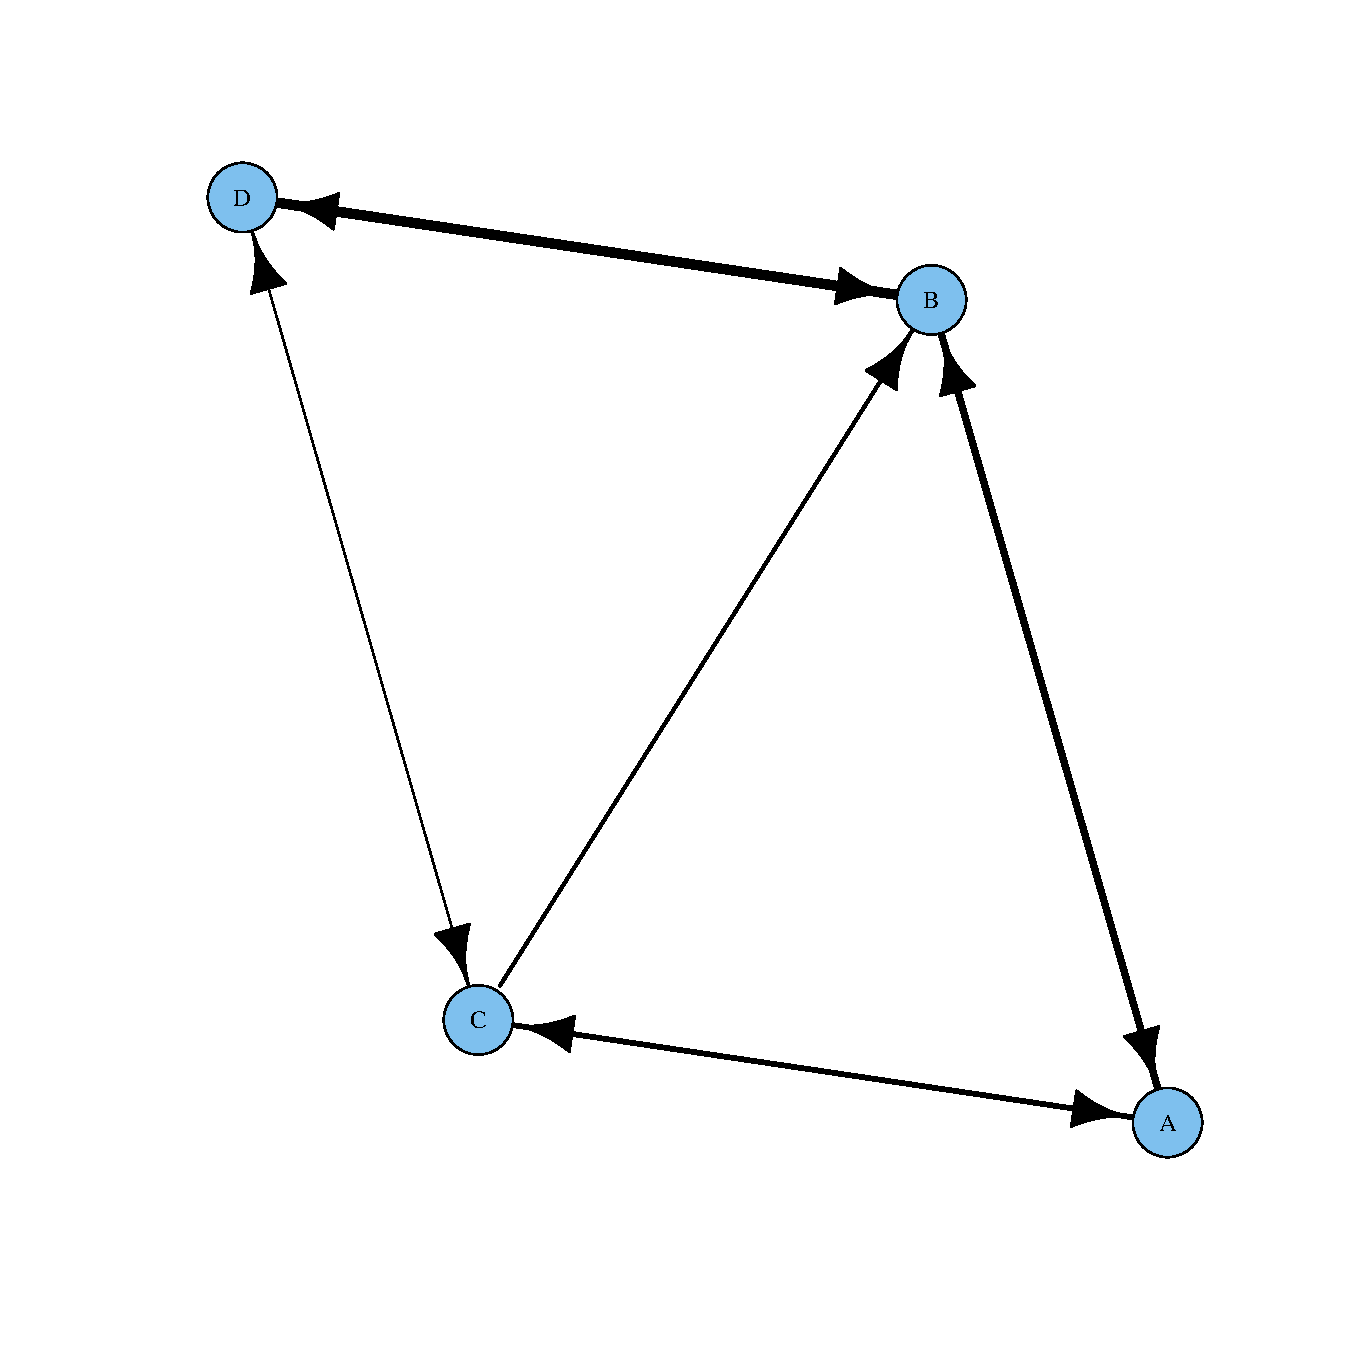
\includegraphics[width=7cm]{fig/metode/moneca_eksempel1.pdf}
}
\parbox[H]{8cm}{\null
\centering
  % \vskip-\abovecaptionskip
  \captionof{table}[Eksempel på vægtet adjacency matrice]{Eksempel på vægtet adjacency matrice}%
  \label{monecaeksempel1.2} 
  \vskip\abovecaptionskip
\begin{tabular}{@{}c|c|c|c|c@{}}
\multicolumn{1}{l|}{} & A & B & C & D \\ \midrule
A                     & - & - & - & - \\ \midrule
B                     & 4 & - & - & - \\ \midrule
C                     & 3 & 2 & - & - \\ \midrule
D                     & 0 & 6 & 1 & -
\end{tabular}
}
\end{figure}
%
Moneca ville i dette tilfælde komme frem til at netværket i figur \ref{monecaeksempel1} består af klyngerne [A|C] og [B|D]. Det sker ud fra følgende procedure: 
%
\begin{enumerate} \label{metode_monecastepbystep}
\itemsep -0.3em
  \item Først lægges de to kraftigst forbundne noder sammen. Det vil her sige [B|D], hvor styrken af forbindelsen er seks.
  \item Derefter gør det den samme med de to næstmest forbunned noder, [A|B], der har en styrke på 4. Eftersom [B] allerede er en del af den foreløbige klynge [B|D], spørger Moneca om det er muligt at indlemme [A] i den allerede etablerede foreløbige klynge. Det kan ikke lade sig gøre, da [A|B] ikke er forbundne.
  \item Moneca går derfor videre til den tredje stærkeste forbindelse, [A|C]. Hverken [A] eller [C] er en del af en foreløbig klynge, og de lægges derfor sammen.
  \item Den fjerde stærkeste forbindelse er [B|C]. [B] og [C] er allerede parret med henholds [D] og [A], og Moneca beregner derfor om [A|B|C|D] udgør en klike, altså alle er forbundne med hinanden. Da det ikke er tilfældet, stopper Moneca og har dermed etableret klyngerne [A|C] og [B|D].
\end{enumerate}
% lidt usikker på om nedenstående bør tages med - det er jo beskrevet heroppe. Måske dobbeltkonfekt. 
Det vil sige at Moneca ikke etablerer nogen af de maksimale kliker, [A|B|C] eller [B|C|D]. Den semistrenge stopregel om klike-tilhørsforhold indenfor klynger betyder desuden, at man med en vis sindsro kan sige at en klynge rent faktisk \emph{er} en samlet størrelse - da den kun kan dannes hvis alle noderne har forbindelse til hinanden, hvilket eksemplet illustrerer: De to maksimale kliker etableres netop ikke, og hvis de gjorde, ville troværdigheden af grænsedragningen mellem klyngerne være langt mere tvivlsom.

For at gentage ovenstående, med andre ord: Moneca starter med at slå noderne med de to mest intense forbindelser sammen til en foreløbig klynge, og går derefter videre til den næstmest intense forbindelse. Hvis en eller begge af noderne i de efterfølgende forbindelser allerede har forbindelse til en tredje eller fjerde node, vurderer Moneca, om denne indgår i en klike med den allerede etablerede klynge. Det er her vigtigt at understrege, at denne vurdering ikke er baseret på styrken af forbindelserne, men udelukkende om der eksisterer en forbindelse%
%
\footnote{Man kan forestille sig en fremtidig version af Moneca foretage en mere avanceret vurdering i disse tvivlsspørgsmål, hvori styrken af relationen kunne indgå som vurderingsgrundlag.}
%
. Moneca fortsætter med denne procedure i prioriteret rækkefølge fra de mest intense forbindelser til de mindst intense, indtil alle noder er placeret i kliker med andre noder, der endnu ikke er “optaget” af en mere intens forbindelse. Kriteriet for, om Moneca tillader at slå de tre noder sammen, er om de tilsammen former en klike, altså alle er forbundet til hinanden. Hvis de ikke er det, går den videre til den den næstmest intense forbindelse, og fortsætter med at forbinde noder indtil der ikke længere kan etableres flere kliker. Kriteriet om at allerede-etablerede klynger kun kan lægges sammen med nye noder, hvis disse indgår i en klike med alle medlemmer af klyngen, er den stop-regel, der gør at Moneca ikke bare ender med at etablere det redundante stykke information, at hvert enkelt komponent%
%
\footnote{Et komponent betyder en subgraf, hvor alle noder er forbundne gennem stier. Et netværk kan således bestå af flere komponenter, der per definition ikke er forbundne (ellers ville de være en del af samme komponent), samt noder uden forbindelse til andre noder (\emph{isolates}) \parencite[100]{Scott2000}.}% 
er en klynge i sig selv \parencite[8]{Touboel2015}. 

Efter denne  første segmentering er Moneca beregnet til at gentage proceduren, indtil det ikke længere er muligt at skabe større klynger. 

Moneca vil gentage denne procedure med de nydannede klynger, der nu behandles som noder i sig selv. Moneca vil i de efterfølgende klyngeinddelinger baseret den på side \pageref{monecastepbystep} beskrevne procedure, \emph{ikke} længere tager de oprindelige, interne forbindelser mellem noderne i betragtning, hvis disse er blevet lagt sammen med andre noder. I den efterfølgende klyngeinddeling vil de interne forbindelser mellem noderne på et lavere niveau ikke indgå i beregningerne i forbindelserne mellem de nyskabte noder. Det vil sige at klike-reglen kun tager højde for forbindelser til noder \emph{på det niveau noderne befinder sig på, og ikke forbindelserne på de lavere niveauer}. 

Når man vurderer kvaliteten af klyngerne på de højere niveauer, er det derfor centralt at se på en række standardmål for klyngens interne forbindelser, for at vurdere rimeligheden af at vurdere klyngen som en samlet størrelse. Det er dette spørgsmål jeg nu afslutter gennemgangen af Moneca med.



% en lang række fordele ved at have fuld population i netværk, udover det argument jeg brugte i adelsbogen, så også fx beregning af densitet (scott s. 74-5) mm. 






%%%%%%%%%%%%%%%%%%%%%%%%%%%%%%%%%%%%%%%%%%%%%%%%%%%%%%%%%%%
\subsection{Opsummering \label{}}
%%%%%%%%%%%%%%%%%%%%%%%%%%%%%%%%%%%%%%%%%%%%%%%%%%%%%%%%%%%

Lorem ipsum dolor sit amet, consectetur adipisicing elit, sed do eiusmod
tempor incididunt ut labore et dolore magna aliqua. Ut enim ad minim veniam,
quis nostrud exercitation ullamco laboris nisi ut aliquip ex ea commodo
consequat. Duis aute irure dolor in reprehenderit in voluptate velit esse
cillum dolore eu fugiat nulla pariatur. Excepteur sint occaecat cupidatat non
proident, sunt in culpa qui officia deserunt mollit anim id est laborum.

Lorem ipsum dolor sit amet, consectetur adipisicing elit, sed do eiusmod
tempor incididunt ut labore et dolore magna aliqua. Ut enim ad minim veniam,
quis nostrud exercitation ullamco laboris nisi ut aliquip ex ea commodo
consequat. Duis aute irure dolor in reprehenderit in voluptate velit esse
cillum dolore eu fugiat nulla pariatur. Excepteur sint occaecat cupidatat non
proident, sunt in culpa qui officia deserunt mollit anim id est laborum.

Efter denne gennemgang af Monecas klyngeinddeling, vil jeg nu gå til det registerdata, der er baggrund for min jobmobilitetsmatrice. Det er temaet for kapitel \ref{kapitel_metode_datamateriale}



\iffalse \label{iffalse}
%%%%%%%%%%%%%%%%%%%%%%%%%%%%%%%%%%%%%%%%%%%%%%%%%%%%%%%%%%%
% Trash 

%%%%%%%%%%%%%%%%%%%%%%%%%%%%%%%%%%%%%%%%%%%%%%%%%%%%%%%%%%%



% Her ville noderne blive bestemt ud fra en given klasseinddeling af interesse, og relationerne mellem disse klasser defineres som ægteskaber. I netværksterminologi betegnes kategorierne som \emph{noder}, mens relationerne mellem noderne betegnes som \emph{edges}, eller på dansk: forbindelser.%
% %
% \footnote{Det er ofte en udfordring at oversætte de tekniske termer fra netværksanalyse til dansk. Hvor det ikke har været muligt  at benytte et tilstrækkeligt unikt oversat dansk begreb, har jeg derfor beholdt de engelske termer.}%
% %
% . I vores speciale ligger jeg derfor konceptuelt helt lig Toubøl \& Larsen, når jeg definerer vores noder som beskæftigelseskategorier, og edges som skift mellem disse kategorier%
% %
% \footnote{Omend forskellen i populationsdefinition - ledige fremfor alle beskæftigede - har stor betydning for den konkrete operationalisering af begreberne, hvilket vil blive behandlet i de efterfølgende kapitler.}%
% %
% . 


% Det centrale er derfor hvilke noder, der benyttes, samt hvad der tæller som en relation mellem to noder. Toubøl og Larsen kommer selv med andre forslag til mulige anvendelser af Moneca, eksempelvis kortlægning af klassemobilitet gennem ægteskaber \parencite[27]{Touboel2013}. 









\fi
%%%%%%%%%%%%%%%%%%%%%%%%%%%%%%%%%%%%%%%%%%%%%%%%%%%%%%%%%%%

%Local Variables: 
%mode: latex
%TeX-master: "report"
%End: